Indexing in databases …..
Indexing would dramatically influence efficient data manipulation and storage [survay]. Like any other type of data, Geo Spatial data would be needed o be indexed. 
Conventional index types are not suitable to support the spatial data [indexing survay], since the spatial data are very large and also complex in structure and relations, operators used for data retrieval are complicated, and spatial orderings would be hard to define. Another point which makes the traditional indices not suitable for spatial objects is that they would consider the spatial objects in one dimension and do not preserve the spatial proximity.
Also, the ordering structures and algorithms for the Geo spatial data should be different from the common data, as …

As it is examined in [survey] many number of spatial indexes has been introduced to improve the spatial data retrieval. Each class and approach has its own strengths and weaknesses and it mostly depends on different issues that based on them is developed, such as requirements, query types, and applications. The classification could be based on different aspect. For example, based on the index structure, the groups would be binary trees, B-Trees, hashing, and space filling methods.
….

Here we discuss some of the approaches from the groups mentioned abow, considering the aspects covered by them.

\subsection{Binary-tree Based}
The indexes in this group are basically and conceptually derived from the binary search tree. They adopt and generalize the idea of partitioning the space. Here some of them are explained.

\subsubsection{The kd-Tree}
This index, which was first introduced by Bentley \cite{bently1975}, is a binary search tree structure for organizing k-dimensional points. As it is explained in \cite{bently1975}, the basic idea is alternatively split the area by x- and y-coordinate, that at each level splits the points half in left, half in right, half below, and half above respectively. For every non-leaf node, there is a k-th dimension discriminator, which defines the the left and right subtrees order association with this node. If the discriminator is associated to the i-th dimension, all the i-th attribute of the sub-nodes in left subtrees are smaller than this node, and all the right sub-tree nodes have the i-th attribute greater.

\begin{figure}
\centering
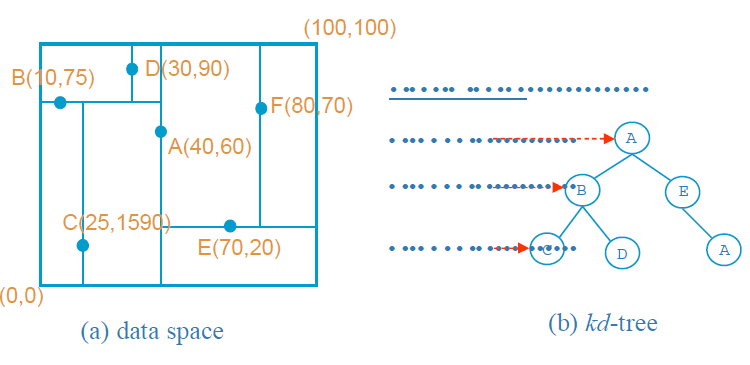
\includegraphics[width=\textwidth]{kdtree}
\caption{kd-tree}
\label{fig1}
\end{figure}


When an item is deleted, a node from the sub-tree must be replaced. Here arises a complication that based on the discriminator in that level, let's call it i, either the node with the smallest i in right sub-tree should be replace or  the node with the biggest i in left sub-tree. A non-homogeneous kd-tree was proposed to make this process cheaper. 
Kd-Tree has been used a lot in intensive searches, but some variants has been introduced to make a better performance in clustering, searching, storage efficiency and balancing [survay], such as …..
and below we discuss some of them.

\subsubsection{Kd-tree Extensions with Paging Capability}
Main memory storage of the index trees are mostly a problem, since it is too big to be placed there  [survay]. Hence, the storage has to be done into disk space. Using binary search tree paging techniques [CeS82 survay] or tree organization of B-trees [BaM72 survay] to store the kd-Tree proposes new indexing structures.

\subsubsection{KDB-tree}
Using properties of both kd-tree and B-tree, the KDB-tree rebuilds the kd-tree to improve some inefficiencies of it.  It means benefits of the balanced kd-trees and the I/O efficiency of B-trees are together. It uses the disk space to bring the kd-tree on disk. 
The method which is used to build  KDB-tree is a space partitioning structure such that the partitions do not overlap each other. The partitions which stand for pages as organizational units, are organized in k-d-tree structure. 
KDB-tree has two basic structures: region page, consist of (region, pageID) pairs, and point page, consist of  (point, pageID) pairs. The region page contains the description of its subpages and a reference to those pages. The point pages contains actual data and references to them. 

\begin{figure}
\centering
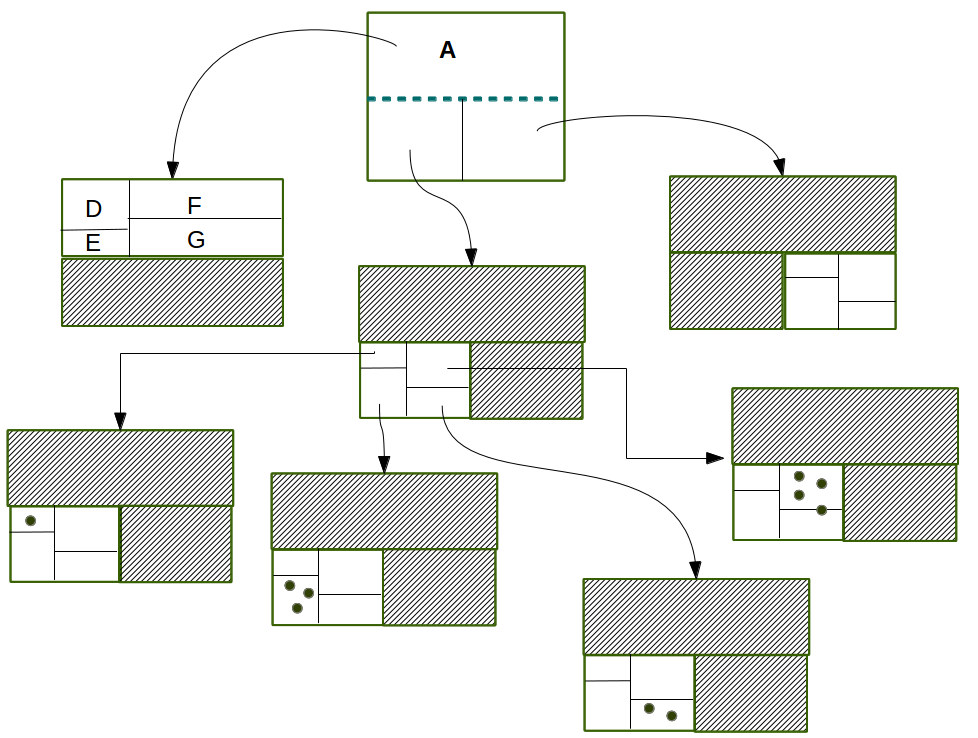
\includegraphics[width=\textwidth]{kdbtree}
\caption{kdb-tree}
\label{fig1}
\end{figure}

The pagination of the B-tree is integrated in the KDB-tree and consequently the tree is height-balanced. Space utilization and efficiency might be low or high, though, since the downward propagation of splitting, caused by region split, may cause low storage utilization. On the other side, there is no guarantee for minimum space utilization. Since partitions do not overlap, it is not always easy to find disjoint partitions to divide a region. So, those partitions must be split at the same value as parent, even though they do not use the minimum amount of space specified for each node. By this problem the range queries' performance is poor. 

\subsubsection{HB-tree}
This is a variation of K-D-B-Tree which could be distinguished by two features: …
Since in a the region split in lower levels result in sparse nodes, hB-Tree (the holey brick Btree) as a multi-attribute index structure is proposed. Data spaces could be holey. It allows the data space associated with a node to be non-rectangular and it uses kd-trees for space representation in its internal nodes. The leaf nodes are known as data nodes and the internal node as index nodes. An index node data space is a union of its child node subspaces which are obtained through kd-tree recursive partitioning. It is height balanced since it is based on the K-D-B-Tree. 
Advantages of this structure is removing the sparse nodes of the K-D-B-Tree and reduction of search time and space utilization, since kd-tree is used. 
Disadvantages of this structure is that the deletion and splitting of nodes are expensive and also multiple references to a data node will lead to more than one traversal of a path.

\begin{figure}
\centering
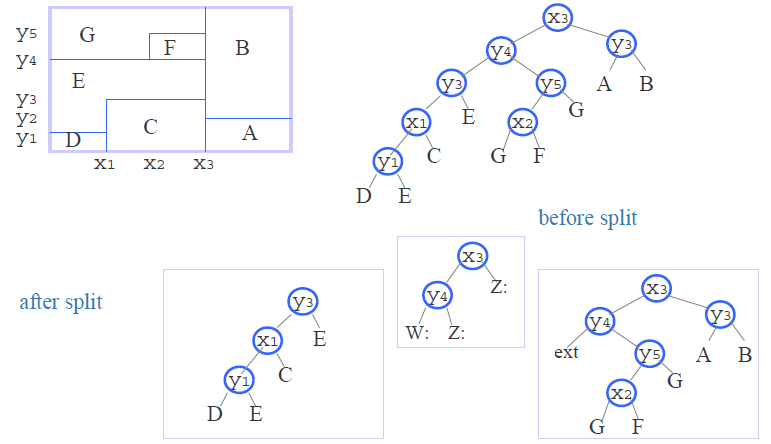
\includegraphics[width=\textwidth]{hbtree}
\caption{hb-tree}
\label{fig1}
\end{figure}

\subsubsection{Matsuyama’s kd-Tree}
This structure is introduced for non-point objects and an extensive duplication strategy is used. The directory is a kd-Tree and a data page is associated for each leaf and those objects which overlaps multiple data spaces are identified in data page and also duplicates. Hence, the data page contains identifiers of the objects totally or partially contained in the corresponding data space.
The point is that this structure is not suitable for large objects since duplication and redundant storage of objects would result in high overhead.

\subsubsection{4D-tree}
Indexes rectangular objects using kd-tree by mapping the objects into points in a four-dimensional space. Each 2D rectangle with (x1, y1) and (x2, y2) is considered as a 4D (x1, y1, x2, y2). As kd-tree the discriminators are chosen cyclically from this set. For each node, a discriminator, discriminator value and pointers to two children are stored. 
For a region search (qx 1, qx 2, qy 1, qy 2), depending on the discriminator, one of the x1 <= qx2, x2  >=  qx1, y1 <= qy2 or y2 >= qy1 has to be done to determine which subtree (or both) has to be searched.
The major problem associated with the 4-d-tree is its intersection search, which can be very costly due to the need for traversal of both subtrees when a query region lies in a subspace that cannot not bounded tightly using the discriminator values.

\subsubsection{skd-tree}
The spatial kd-Tree alters the kd-tree in a way that objects are indexed by their centroid and the minimum bounding box of the object is also stored in the node. This structure is suitable for non-point spatial objects. In a kd-tree the objects which are contained in more than one space, will be referenced more than once. To avoid the duplication virtual subspaces are defined which include the original subspaces. So, each object are placed in the subspace based on its centroid.
With this devision, we just need one more value for each subspace which shows min/max values along the dimension of the discriminator. Therefore, the structure of each node would consist of:
Two children
The discriminator and it's value
The max/ min value of objects left(LOSON)/right(HISON) subspaces along with dimension of the discriminator
The maximum/minimum value of LOSON/HISON the nearest virtual line which bounds the data whose centroid are inside the LOSON/HISON.

\begin{figure}
\centering
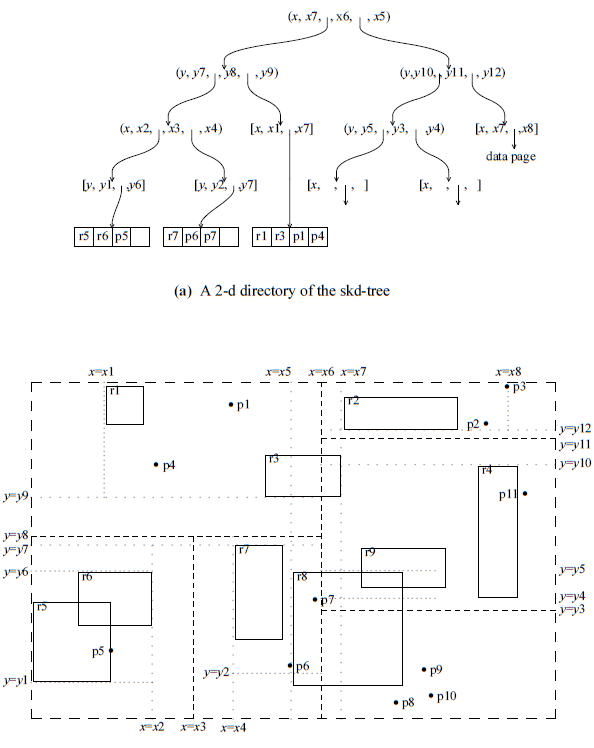
\includegraphics[width=\textwidth]{skdtree}
\caption{skd-tree}
\label{fig1}
\end{figure}

During traversal a rectangular space is associated with each node and materialized  such that is tested against the query region if it intersects the region. 
(Since the virtual boundary may sometimes bound the objects tighter than the partitioning line, the intersection search takes advantage of the existing virtual boundary to prune the search space efficiently. To further exploit the virtual boundaries, containment search which retrieves all spatial objects contained in a given query rectangle was proposed. During tree traversal, the algorithm always selects the boundaries that yield smaller search space. The direct support of containment search is useful to operators like within and contain. The search rapidly eliminates all objects that are not totally contained in the query region.)
The Sdk-tree is memory-based, not a disk-based, data structure, thus is not suitable for very large databases.

\subsection{B-tree based Indexing Technique}
\subsubsection{R-tree}

Minimization of both coverage and overlap is crucial to the performance of R-trees.
\subsubsection{$R^*$-tree}
The $R^*$-tree is found to be more efficient than some other variants, and the R-tree using linear splitting algorithm is substantially less efficient than the one with quadratic splitting algorithm. In general, the R*-tree is an improvement over the R-tree at the expense of more expensive insertion.

This structure tries to reduce overlaps between directory rectangles and the area covered by a rectangle, in order to make better performance, since minimum overlaps leads to less number of branches to be traversed in queries and minimum coverage helps to decide on the paths to traverse on higher levels. 
R*-Tree does these optimizations with revised node split and also forced insertion which finds a better place for a node that its original place. In R-Tree insertion-build structure is highly suboptimal and insertion and deletion could improves the R-Tree dramatically.
 (Using the idea of reinsertion of the R-tree, Beckmann et al proposed a reinsertion algorithm when a node overflows. The reinsertion sorts the entries in decreasing order of the distance between the centroids of the rectangle and the covering rectangle and reinserts the first p (variable for tuning) entries. In some cases, the entries are reinserted back into the same node and hence a split is eventually necessary. The reinsertion will no doubt increase the storage utilization; but it can be fairly expensive when the tree is large. The R*-tree is found to be more efficient than some other variants, and the R-tree using linear splitting algorithm is substantially less efficient than the one with quadratic splitting algorithm. In general, the R*-tree is an improvement over the R-tree at the expense of more expensive insertion.)

\subsubsection{The Buddy Tree}
(In comparison to previously proposed tree structures such as the K-D-B-tree, the buddy-tree guarantees a more efficient dynamic behavior.Moreover, indirect splits which cause low storage utilization and high insertion costs in the K-D-B-tree, are completely avoided. This structure is 
It avoids the downward splitting of the K-DB-tree, the overlapping problem of the R-tree and the dependency of structures upon the insertion of data. The buddy-tree generalizes the buddy system of the grid-file to organize correlated data efficiently, by bounding the data points tightly using the bounding rectangle concepts of the R-tree and organize the directory as in the R-tree. Like grid-files, the non-zero sized data have to be mapped into higher dimension.
An important feature of the buddy-tree is that it does not partition empty data space. Therefore queries, such as partial match queries, where the query region intersects with empty data space, can be performed much faster than by conventional structures partitioning the complete data space.
The following summarizes the design properties of the buddy-tree:
empty data space is not partitioned
insertion and deletion of a record is restricted to
exactly one path
no overflow pages
directory grows linear in the number of records
performance is basicly independent of the sequence of
insertions
efficient behavior for insertions and deletions
very high fan out of the directory nodes)

\subsubsection{The Packed R-Tree}

In order to minimize storage space, coverages and overlaps in R-Tree, constructing a static tree is proposed. To make this tree, first the objects are ordered along a coordinate. The object with the minimum value then is chosen to find the M nearest objects to that one, and assigns them to a node. Here M is the maximum number of objects that are allowed in a page. This step is repeated until the whole objects are assigned to a node. The bounding box of the leaf nodes are higher level objects. These are also ordered and assigned to the nodes. The process repeats until the number of the remained nodes is less than M. If so, they are assigned to the root.
The main objective of the algorithm is to reduce the storage space, the coverage and overlap of rectangles, in order to improve the search efficiency.

\subsubsection{R+-Tree}

This structure is a compromise between the R-tree and the K-D-B-tree, to solve the overlapping problem of covering rectangles. It has just some difference:

Nodes of an R+-tree are not guaranteed to be at least half filled.
 The entries of any intermediate (internal) node do not overlap.
 An object identifier may be stored in more than one leaf node.

The duplication of the objects in the tree avoids overlappings and consequently leads to less path traversals in point queries. 
On the other hand there is some disadvantages: it might be bigger that R-Tree as a result of duplications, and the construction and maintenance are more complex that R-Tree or other variants. 
Also, in insertion cases into the tree a case would happen that the	covering rectangles of some entries can prevent each other from expanding to include the new object. In other words, some space ("dead space") within the current node cannot be covered by any of the covering rectangles of the entries in the node. If the new object occupies such a region, it cannot be fully covered by the entries. When a new object cannot be fully covered, one or more of the covering rectangles are split. This means that the split may cause the children of the entries to be split as well, which may further degrade the storage efficiency.
In performance study, in the comparison between R-trees and R+-trees, it is found that the R+-tree requires much more splits, especially for large data objects, but lesser splits for smaller data objects. 
In general, the query efficiency tests show that R+-trees perform better for smaller objects and slightly worse off for larger objects.

\subsubsection{STR-tree}

\subsubsection{Cell-tree}
The cell tree introduces a structure to overcome the overlapping bounding rectangle problems of R-trees and the "dead space" (empty space) problems of R+-trees. Partitioning is done in a recursive way, but not necessarily with rectangles. Instead, the regions are polyhedral, as bounding polygons. Subspaces do not overlap.  
\begin{figure}
\centering
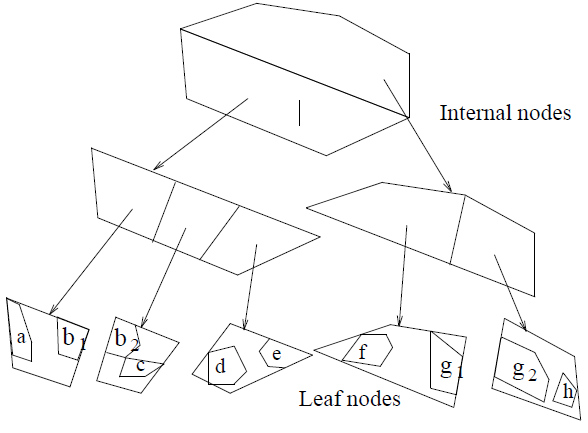
\includegraphics[width=\textwidth]{celltree}
\caption{cell-tree}
\label{fig1}
\end{figure}

Like R+-Tree, objects might be represented in more than one leaf node. One problem with such an instruction which duplicates the objects is that each new object may be divided into multiple pieces in order to store them in a tree where internal node bounding polygons do not overlap. Specially in populated DBs. 
(Each split of a node leads to a decrease in the node data space but to an increase in the number of nodes per object. To overcome the fragmentation and duplication problems, Gunther and Noltemeier proposed to store oversized objects which may greatly increase the number of object identifiers being stored in the leaf nodes in separate "oversize shelves". These oversize shelves are data nodes linked to internal nodes in the cell-tree, in one way, causing the tree to be not height-balanced. The placement of a new object in the subtree or oversize shelf requires some optimization. The oversize page shelf can be overflowed and a split on this shelf is necessary.)
\subsubsection{Quadtree}
It is organized in a way similar to the region quad-tree. A region is recursively partitioned until the resulting quadrants do not contain any rectangle. During the subdivision, all rectangles that intersect with either of the two partitioning lines are associated with the partitioning lines. The rectangles that are associated with a quadrant must not belong to any ancestor quadrant. It is assumed that no two rectangles overlap.
